\subsection{Fluidodinamica}

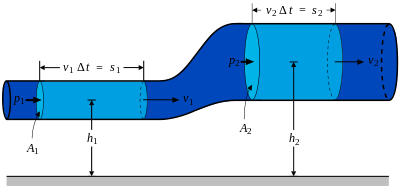
\includegraphics[width=1 \linewidth]{FluidoDinamica/flusso.png} \\

\begin{gather*}
    \text{Densità(massa volumica): } \rho = \frac{m}{V} \\
    \text{Massa: } m = \rho V \\
    \text{Volume: } V = \frac{m}{\rho} \\
    \text{Teorema di Bernoulli: } \\ p_1 + \frac{1}{2} \rho v_1^2 + \rho g h_1 = p_2 + \frac{1}{2} \rho v_2^2 + \rho g h_2 \\
    \text{Equazione di Continuità(ideale): } \\  Q = v_1 S_1 = v_2 S_2 \\
    \text{Equazione di Continuità(reale): } \\ Q = \rho_1 v_1 S_1 = \rho_1 v_2 S_2 \\
    \text{Velocità 1: } v_1 = \frac{Q}{S_1} = \frac{S_2}{S_1} v_2 \\
    \text{Velocità 2: } v_2 = \frac{Q}{S_2} = \frac{S_1}{S_2} v_1 \\
    \text{Sezione 1: } S_1 = \frac{v_2}{v_1} S_2 \\
    \text{Sezione 2: } S_2 = \frac{v_1}{v_2} S_1 \\\
    \text{Differenza di pressione: } \\
    \Delta p = \frac{1}{2} \rho (v_2^2 - v_1^2) \\ 
    \Delta p = \frac{1}{2} \rho (\frac{Q^2}{S_2^2} - \frac{Q^2}{S_1^2})
\end{gather*}